\subsection{Sorting}
Sorting algorithms are used to reorder elements in a datastructure, often arrays or lists. The elements are ordered by a rule depending on what type of element the datastructure contains. Numbers are often ordered from the lowest number to the largest. Characters are often ordered by transforming the character into a number, where "a" is often defined as smaller than "b".
\\[11pt]
To sort the elements an algorithm must be used. They have different performance and memory usage so it's important to be able to pick the best fitting algorithm depending on the situation. This project contains implementations of insertion sort, shell sort, merge sort and quick sort which are common algorithms. They are written to work on arrays containing any element which can be compared using the >, < and == operators in JavaScript. Instead of returning the sorted version of an array, they return functions which can be called to navigate between the steps of the algorithm. When checking if an student's answer is correct it's pointless to check if they managed to sort the array, because they might not have sorted the array according to the rules of the algorithm. The steps are therefore returned, so that together with the GraphDrawer, the students can graphically perform the sort. It is then possible to compare each step with what the student did and see if they know how the algorithm works.

\subsubsection{Insertion Sort}
Insertion sort is simplest sorting algorithm learned in the algorithms and data structures course. Insertion sort uses an easy algorithm that is forced to go though every entry in a list. The algorithm checks whether or not the current entry has a smaller value then the previous entry, if entry has a smaller value, then the previous entries have to re-sorted with the entry until either you find an entry that is smaller or reach the start of the list. 
\\[11pt]
The insertion sort is quite easy to implement, essentially only consists of a for-loop and a while-loop. Because its simple design its a sorting algorithm that is quite often used. Insertion sort is however quite slow compared to most other sorting algorithms. It only has an O(n) average run time, and a runtime of O($n^2$) in terms of worst case scenario.
\\[11pt]
Although insertion sort is quite effective when it is used to sort almost fully sorted list's. This means that insertion sort algorithm is used by a lot of other sorting algorithms. Mostly used as a final step in these other sorting algorithms. Examples of this being the sorting algorithms Shell sort, Merge sort and Quick sort.	%Probably have should have a cite to the different sorting algorithms mentioned just now.

\subsection{Shell Sort}
Shell sort is a sorting algorithm that is based on insertion sort. The key difference between the two sorting algorithms is in performance. Shell sort will have both an average case and a worst case of O(n) runtime. The main reason for this is that shell sort will sort entries in the list that are at certain intervals from each other. The algorithm is essentially dividing list entries into smaller sublists in order to make the sorting more efficient. Through this method, shell sort avoids having to check every entry in the list, which allows the algorithm to remove the main drawback of using insertion sort.
\\[11pt]
The starting interval used in a shell sort is usually based on approximately half length of the list. The algorithm uses the interval to divide up the entries in the list. The entries chosen together are then compared to each other and sorted based on their value. Once the list has been effectively sorted on the current k-interval, the interval's value is halved and the sorting process starts anew. Eventually, the interval will reach a value of 1, which causes shell sort to finish sorting the list using the insertion sort algorithm. Of course, since the list should at this point be almost completely sorted, and therefore the insertion sort should never achieve a run-time of $O(n^2)$.

\subsubsection{Merge Sort}
While performing the sort, every stage of the algorithm is saved in a list of steps. There are three stages which are stored as a step.
\begin{itemize}
    \item Initial. The initial step is stored before the sorting starts. It contains a copy of the unsorted array and a reference to the limit.
    \item Split. The split step is added when an array is split into two arrays. It contains a copy of the array being split, and copies of the new arrays.
    \item Merge. The merge step is added after two arrays have been merged to a new array containing the sorted version of all the elements. It contains a copy of the two arrays being merged and a copy of the resulting array.
\end{itemize}
When implementing the algorithm, performance and memory usage were not considered to be important. The algorithm runs only once per question to generate the steps so that each student's answer can be compared to the right way of performing a merge sort. For this reason, the intermediate arrays are allocated dynamically instead of being reused in later steps. This gives the algorithm worse performance, but its average case performance is still $O(n * logn)$. Memory usage has not been considered because the algorithm has to store more information than normal to store the steps.

\subsubsection{Quick Sort}
While performing the sort the algoritm we wrote also stores the state of steps that we picked. This is done for the solution checker to be able to check if the student has drawn the correct answer when simulating the quicksort algorithm.
\begin{itemize}
    \item Initial: The initial step is stored before the sorting starts. It contains a copy of the unsorted array.
    \item Split: The split step is stored each time the algorithm splits a list, it will store the unsorted list that it will split, the pivot point, left and right list.
    \item Merge: The merge step is stored each time the algorithm merges the sorted lists and pivot point. It will store information about the sorted left and right list, the pivot point and the sorted list after the merge.
\end{itemize}
\begin{figure}[H]
    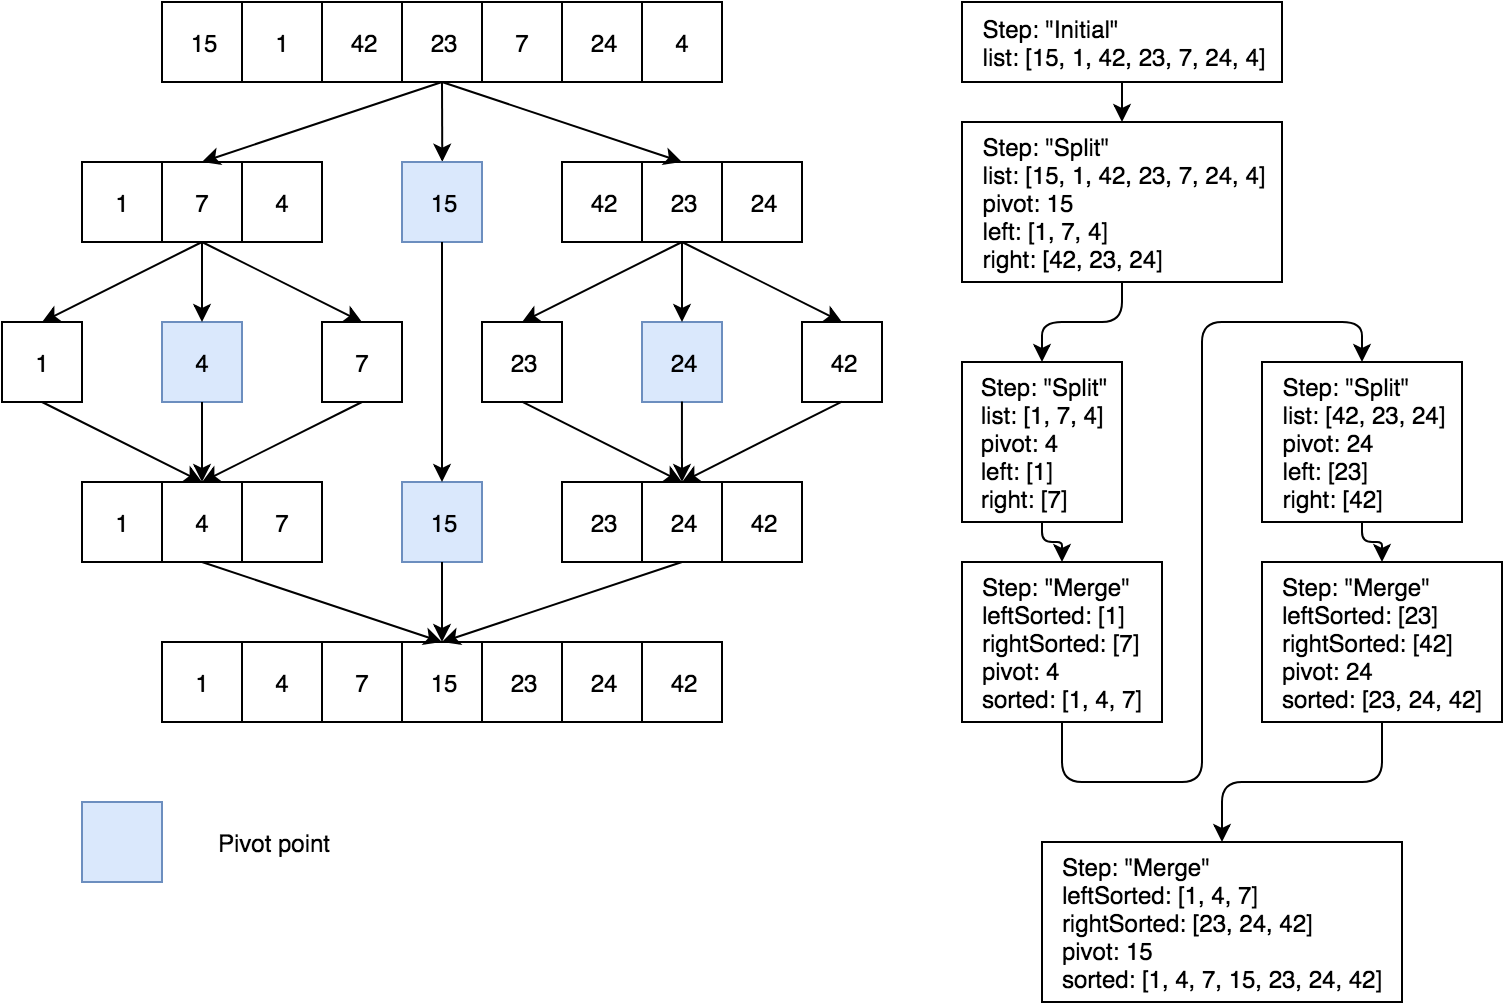
\includegraphics[width=\linewidth]{/diagrammer/Quicksort}
    \caption{Quicksort}
    \label{fig:quicksort}
\end{figure}
